\documentclass[times,twocolumn,final]{elsarticle}

\usepackage{cag}
\usepackage{framed,multirow}
\usepackage{amssymb}
\usepackage{amsmath}
\usepackage{lineno}
\usepackage{graphicx}
\usepackage{booktabs}
\usepackage{placeins}
\setcounter{totalnumber}{6}
\setcounter{topnumber}{4}
\setcounter{bottomnumber}{4}
\renewcommand{\topfraction}{0.92}
\renewcommand{\textfraction}{0.05}
\renewcommand{\floatpagefraction}{0.85}


\journal{Computers \& Graphics}

\begin{document}

\begin{frontmatter}

\title{Timestep-Conditioned Adapter Scaling for Multi-view Diffusion Texture Generation}

% Double-anonymized review: author names, affiliations, and acknowledgements
% (including funding) are provided only on the separately uploaded title page.

\begin{abstract}
Geometry-adapter strength is a practical inference-time control in multi-view texture generation: scaling its residual changes the influence of shape constraints on generated views and may also change appearance. We operationalize this control as Timestep-Conditioned Adapter Scaling (TCAS), a training-free, piecewise requested-scale profile on an existing geometry-adapter residual. TCAS keeps requested scales distinct from values applied under the wrapper's native caps and from the resulting residual magnitudes; we evaluate the recorded C3 profile, $(1.25,2.50,1.25)$. In a matched held-out image-space study on 300 objects, C3 improves mean foreground PSNR over global fixed-low scaling (GFL) by $+0.522352$~dB (95\% object-bootstrap CI $[+0.404160,+0.640669]$). This result is bounded: global fixed-high scaling (GFH) and Generic Linear have more favorable cohort means than C3 on all four displayed endpoints. Moreover, C3 and GFL have applied deep/middle scale sums of 82.5 and 62.5 per layer, respectively, while both have a shallow sum of 40; the contrast therefore does not isolate a pure timing effect. In a separate post-inspection 276-object stage-placement follow-up, C3 exceeds a fixed-mean profile by $+0.502875$~dB FG-PSNR; the C3-minus-temporal-L--L--H FG-PSNR difference is $-0.177084$~dB, and temporal L--L--H outperforms C3 on all six formal endpoints. These studies show response sensitivity to the tested profiles, not an equal-residual-dose mechanism or an optimal schedule. The evidence concerns rendered images and does not establish baked-texture, seam, PBR, or general cross-backbone improvement.
\end{abstract}

\begin{keyword}
\KWD
multi-view diffusion model \sep 3D texture generation \sep adapter scaling \sep timestep-conditioned scaling \sep shape-texture trade-off \sep geometric control
\end{keyword}

\end{frontmatter}

\linenumbers

\section{Introduction}
\label{sec:intro}

Multi-view diffusion systems generate target-view images that can later be projected or baked onto a 3D surface. In geometry-conditioned systems, an adapter injects shape information into the denoiser through intermediate residuals. The strength applied to those residuals is therefore a practical inference-time control: changing it can alter how strongly geometry conditions the generated views and can also change their appearance. The useful setting depends on the adapter implementation and on the image endpoint being considered, so a single structural score cannot characterize the full effect.

This paper studies that control question in a fixed MVPainter-style multi-view texturing pipeline. Timestep-Conditioned Adapter Scaling (TCAS) applies a piecewise requested-scale profile to the existing GeoTex-Adapter residual path without training parameters or changing model weights. We examine the recorded C3 profile, $(1.25,2.50,1.25)$, and distinguish its requested values from the values applied by the wrapper's native caps and from the resulting residual magnitudes. This makes the intervention executable and its limits measurable.

Time-varying control is an established idea. Scheduled Style Injection (SSI) studies schedules across decoder layers and denoising time for style injection and also schedules geometry-conditioned ControlNet strength. TCAS does not claim a new general scheduling primitive. It asks a narrower question about the requested temporal scale of a geometry-adapter residual in multi-view texture generation, and evaluates that intervention under a matched image-space protocol. The task, conditioning interface, and endpoints differ from SSI, so their quantitative results are not directly comparable.

We evaluate C3 on a 300-object held-out cohort against fixed and scheduled controls. The positive C3--GFL foreground-PSNR result is presented alongside GFH and Generic Linear counter-results, and we report the applied-scale difference that prevents interpreting C3--GFL as a timing-only contrast. Separate stage-placement and layer-window studies examine response variation under tested profiles. They show that outcomes depend on the profile and endpoint, but do not establish dose-independent scheduling or a universally preferred schedule. All current Fresh C endpoints are image-space measures; they do not establish material fidelity after baking.

The contributions are:

(1) We specify TCAS as a training-free, three-stage requested-scale intervention on an existing geometry-adapter residual, with requested, applied, capped, and residual-magnitude quantities kept distinct.

(2) We report a matched 300-object comparison in which C3 exceeds GFL on the registered FG-PSNR endpoint, while GFH and Generic Linear have more favorable means than C3 on all four displayed endpoints. The differing applied-scale sums delimit the interpretation of the C3--GFL contrast.

(3) We examine profile sensitivity with separate temporal-placement, layer-window, and cross-interface analyses. The results show response differences under the tested settings, while cohort, realized-dose, and interface limits leave dose-independent causality and general transfer unresolved.

\section{Related Work}
\label{sec:related}

\subsection{3D Texture Generation and Multi-view Diffusion}
\label{subsec:3dtex}

Single-image 3D generation is often decomposed into geometry generation and texture generation. Single-image-to-3D, multi-view diffusion, and sparse-view reconstruction methods have improved structural stability and view synthesis \cite{liu2023zero1to3,shi2023zero123pp,liu2023syncdreamer,long2023wonder3d,shi2024mvdream,wang2023imagedream,xu2024instantmesh,ke2024era3d}. Texture synthesis remains a distinct challenge for asset realism and usability \cite{perla2026survey}. Many systems generate RGB views with 2D diffusion and project or bake them onto a surface \cite{chen2023text2tex,richardson2023texture,poole2023dreamfusion,chen2023fantasia3d}. Recent work also explores exemplar-based texture synthesis and diffusion-based procedural materials \cite{guzman2026adaptive,lv2025interpretable}.

Paint3D, MVPaint, Hunyuan3D 2.0, and MVPainter use geometry-conditioned multi-view generation in 3D texturing pipelines \cite{zeng2024paint3d,cheng2024mvpaint,lai2025hunyuan3d,shao2025mvpainter}. MV-Adapter and synchronized multi-view methods address multi-view consistency through different adapter and denoising designs \cite{huang2024mvadapter,liu2024synchronized,xu2026wondertex}. These systems establish the graphics context for this work. The present evidence does not compare final baked-texture quality across those systems.

\subsection{Adapter-Augmented Diffusion Models and Geometric Control}
\label{subsec:adapter}

T2I-Adapter and ControlNet inject spatial conditions into pretrained diffusion models through controllable branches \cite{mou2023t2iadapter,zhang2023controlnet}. IP-Adapter introduces image prompts through decoupled attention \cite{ye2023ipadapter}; LoRA and related methods use scaled low-rank updates \cite{hu2022lora,liu2024dora,zhang2023adalora}. These methods establish condition and residual scaling as common implementation controls. TCAS does not introduce adapter conditioning or a new multi-view backbone; it studies a requested scale on the existing GeoTex-Adapter residual path.

\subsection{Diffusion Guidance Scheduling and Timestep Control}
\label{subsec:guidance}

Diffusion denoising is often discussed in terms of coarse-to-fine evolution, and prior work varies guidance strength over sampling progress to study quality, diversity, or fidelity \cite{ho2020ddpm,song2021ddim,ho2022cfg,castillo2023adaptive}. Limited-interval classifier-free guidance is one example; it changes the combination of conditional and unconditional score predictions \cite{kynkanniemi2024limited}.

Scheduled Style Injection (SSI) is the closest scheduling precedent: it schedules style injection across decoder layers and denoising time and also studies schedules for geometry-conditioned ControlNet strength \cite{kulkarni2026ssi}. Thus, layer-by-time conditioning schedules and time-varying geometry control are established ideas. TCAS is narrower: it applies a three-stage requested multiplier to the GeoTex-Adapter residual in a multi-view texture-generation pipeline. The paper evaluates that task-specific intervention and its implementation boundaries; it does not claim a new general scheduling primitive or first use of layer/time control. SSI and TCAS use different models, interventions, datasets, and endpoints, so their quantitative results are not directly comparable.

\section{Method}
\label{sec:method}

\subsection{Task Definition and Base Pipeline}
\label{subsec:task}

This paper builds on the MVPainter-style geometry-controlled multi-view texture generation framework \cite{shao2025mvpainter} and studies how the inference-time strength of geometric condition injection affects the generated results. Figure~\ref{fig:overview} illustrates the overall pipeline: the adapter injects geometric residuals into UNet features, TCAS adjusts their strength across denoising stages, and the final multi-view outputs are projected and baked into a textured 3D mesh. Given a single reference image and the corresponding 3D geometry, the base pipeline first generates RGB texture images from six target views and then obtains a textured mesh through projection or texture baking. We do not modify the base UNet, VAE, or pretrained adapter weights. Instead, the adapter scaling factor is treated as the key inference-time control variable.

\begin{figure*}[t]
\centering
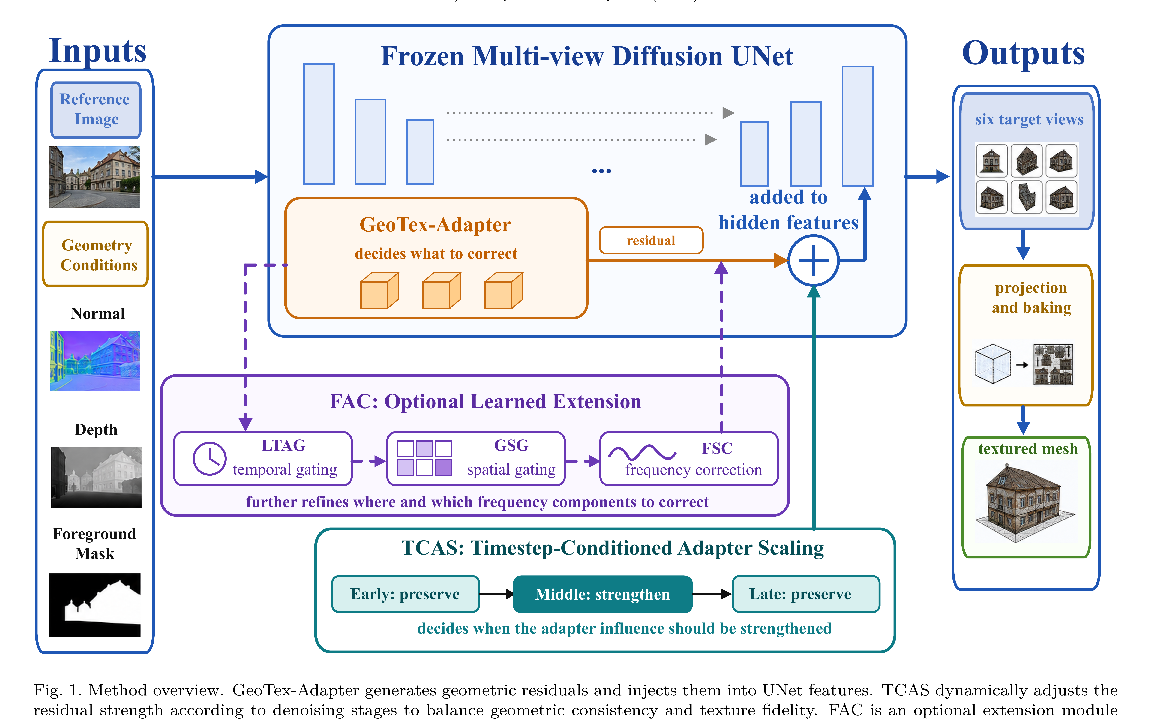
\includegraphics[width=\textwidth,trim=0 24pt 0 0,clip]{figures/fig1_01549_original.pdf}
\caption{Method overview reproduced from the authenticated 01549 submission. The optional FAC branch is retained as a previously reported extension; its controlled negative re-examination from 01549 is summarized in Section~\ref{subsec:facreported}. TCAS remains the paper's training-free method. Projection and baking are pipeline context, not outcomes validated by Fresh C image-space evidence.}
\label{fig:overview}
\end{figure*}

During multi-view diffusion, the 3D geometry is rendered into normal maps, depth maps, and foreground masks, denoted as:
\begin{equation}
\mathbf{G} = \{G_\text{normal}, G_\text{depth}, G_\text{mask}\}.
\end{equation}

The geometric adapter maps these conditions to a residual correction term and injects it into the intermediate hidden states of the UNet. For the $t$-th denoising step, the adapter injection can be written as:
\begin{equation}
\mathbf{h}'_{t,\ell} = \mathbf{h}_{t,\ell} + s_{\mathrm{app}}(p_t,\ell)\, A^\ell_\phi(\mathbf{h}_{t,\ell}, \mathbf{G}),
\label{eq:injection}
\end{equation}
where $\ell$ indexes an injected layer group, $p_t$ is normalized sampling progress, and $s_{\mathrm{app}}$ is the scale actually applied by the wrapper. We distinguish it from the requested profile $s_{\mathrm{req}}$: when a native cap $c_\ell$ is active, $s_{\mathrm{app}}(p_t,\ell)=\min(s_{\mathrm{req}}(p_t,\ell),c_\ell)$; otherwise the wrapper applies the request. The scaled residual's magnitude also depends on $A^\ell_\phi$ and is not determined by the scale label alone. In the Fresh C implementation, the logged caps are 3.0 (deep), 3.5 (middle), and 0.8 (shallow). Thus C3's requested shallow value 1.25 is applied as 0.8, while its deep and middle requests pass unchanged. GFL and GFH also clip at the shallow cap. These cap values describe the audited Fresh C wrapper; row-level cap semantics for the historical 24-object probe are not fully recoverable. TCAS changes a residual added to feature activations, rather than reweighting conditional and unconditional score predictions as CFG does.

\subsection{Image-Space Metrics and Texture-Variation Diagnostics}
\label{subsec:metrics}

We distinguish structure and signal-similarity measures from texture-variation proxies. FG-SSIM, Edge-SSIM, and Crop-SSIM quantify structural similarity on the indicated image regions; PSNR measures pixel error; LPIPS compares learned image features \cite{wang2004ssim,zhang2018lpips}. These endpoints describe agreement with target-view renderings, not complete perceptual or material fidelity.

Laplacian variance, RGB standard deviation, and gradient magnitude can describe local high-frequency or color variation. For example, a foreground Laplacian statistic may be written as
\begin{equation}
M_{\mathrm{var}}=\operatorname{Var}\!\left(\operatorname{Lap}(I_{\mathrm{out}}\odot G_{\mathrm{mask}})\right),
\end{equation}
where $G_{\mathrm{mask}}$ is the foreground mask. A larger value is not necessarily better: detail, noise, repeated patterns, or artifacts can all increase local variation. We therefore do not interpret these proxies as texture fidelity or use them alone to claim that a schedule better preserves reference appearance.

\subsection{Timestep-Conditioned Adapter Scaling}
\label{subsec:tcas}

TCAS replaces a globally fixed requested adapter scale with a piecewise profile over normalized sampling progress. The early/middle/late partition is an operational description, not a universal claim about the function of every denoising stage. C3's low--high--low profile is the specific development choice evaluated in this revision; it is not presented as an independently derived optimum.

To avoid ambiguity caused by different raw timestep directions in different schedulers, we use sampling progress $p$ to represent the denoising process, where $p = 0$ denotes the start from noise and $p = 1$ denotes the end of sampling close to the final image state. TCAS divides denoising into early, middle, and late stages:
\begin{equation}
s_{\mathrm{req}}(p) = \begin{cases} s_e, & 0 \leq p < 1/3 \\ s_m, & 1/3 \leq p < 2/3 \\ s_l, & 2/3 \leq p \leq 1 \end{cases}.
\label{eq:tcas}
\end{equation}

The selected C3 configuration used in this paper is:
\begin{equation}
(s_e, s_m, s_l) = (1.25, 2.50, 1.25).
\end{equation}

The low--high--low profile is a concrete inference-time intervention motivated by the submitted development analysis. Its stage interpretation is a task-specific hypothesis: early, middle, and late sampling may respond differently to geometry residuals. Fresh C evaluates the recorded profile against matched controls but does not prove that each stage has a universal functional role. TCAS adds no trained parameters and does not modify base-model or adapter weights; it replaces the requested scaling value during inference.

\paragraph{Development origin and scope of C3}
The submitted 01549 paper records C3 $=(1.25,2.50,1.25)$ as the selected profile from a 24-object development probe containing 17 uniform, layer-wise, and time-conditioned variants. We retain that development record because it explains the origin of the profile studied here. The complete row-level outputs and selection-time provenance are not available in the current evidence authority, so the historical ranking and labels cannot be independently checked. We therefore make no formal optimality or uniqueness claim based on this probe. Fresh C evaluates the recorded profile without further schedule search.

\subsection{Geometry Adapter and Inference Interface}
\label{subsec:adapterimpl}

GeoTex-Adapter is treated as the fixed geometry-residual backbone, not as a new contribution of this paper. It receives a five-channel input comprising a three-channel normal map, a one-channel depth map, and a one-channel foreground mask. A multi-scale encoder produces residual features that are injected into the frozen UNet. TCAS acts on the requested multiplier along denoising progress; it does not retrain the adapter, the UNet, or the VAE and introduces no learned parameters.

The first-round 01549 revision also reported a learned Full Adaptive Correction (FAC) extension. We retain its controlled negative re-examination as a previously reported auxiliary result in Section~\ref{subsec:facreported} and Supplementary Table~S11; it is not a new 1008 training run. TCAS remains the paper's sole training-free method.

\section{Experiments}
\label{sec:experiments}

\subsection{Experimental Setup}
\label{subsec:setup}

\subsubsection{Experimental protocol and comparisons}

The original 01549 submission reports fixed-scale experiments, a 24-object schedule-development probe, and a 300-object pooled evaluation. The source figures and tables are authentic submission artifacts, but the current evidence archive does not contain a complete object-level manifest and run record for every historical result. We therefore preserve the fixed-scale and C3-selection questions as historical development evidence and do not present their unrecovered numbers as newly verified confirmatory results.

Fresh C is a held-out, matched image-space study on 300 frozen object identifiers, independent of the original 24-object schedule-selection probe and the original 300-object evaluation cohort. The primary four-condition run (No Adapter, GFL, GFH, and C3) and the same-cohort Generic Linear/LLH addendum use the same frozen adapter checkpoint (SHA-256 \texttt{0618d6b2\allowbreak{}84ab47aa\allowbreak{}16d7a89d\allowbreak{}c447f5ba\allowbreak{}4455ff6c\allowbreak{}9d918e5e\allowbreak{}129478a9\allowbreak{}9e0114c0}), runner source (SHA-256 \texttt{e5c28e91\allowbreak{}5ba137d3\allowbreak{}541eb4c0\allowbreak{}32daaf62\allowbreak{}a798332d\allowbreak{}63b32917\allowbreak{}b749fe1b\allowbreak{}cc74e9e3}), 300-object cohort, reference/geometry inputs, target views, metric implementation, and per-object seed policy $42+\texttt{object\_idx}$. The verified gates cover 1,200/1,200 primary rows and 600/600 addendum rows. The registered primary endpoint is paired C3--GFL FG-PSNR. Fresh C's 300 UIDs have zero overlap with the original evaluation cohort (including its probe), the original 1,118-object training list, and the clean-v2 evaluation cohort. The Fresh C comparison uses one frozen checkpoint and common execution protocol; hash identity with the historical Table~4 checkpoint is not used as a validity condition. The historical distinction remains: 01549 names a v1 checkpoint for its main tables and a separate v2 strong-residual, per-layer-capped adapter for Section~4.7/FAC; Fresh C is a controlled retraining, and its estimate is not presented as a numerical reproduction of the old $+0.96$~dB contrast. The separate post-inspection strict-276 analyses use the clean-v2 object list and record the same checkpoint SHA as Fresh C; their cohort and run provenance differ from Fresh C, and they are reported only as bounded supporting diagnostics.

\subsubsection{Evaluation sets and metrics}

The submitted paper describes a 50-object, 13-scale sweep; a purposive 26-object texture audit; a 24-object, 17-variant development probe; and a pooled 300-object evaluation. We retain the 50-object sweep and the 24-object probe as historical diagnostics because they motivate the scale-allocation question. Their object-level raw outputs, full selection provenance, or metric implementation records are incomplete in the current archive. The 26-object audit's object IDs, selection trace, and proxy definitions also cannot be reconstructed; its prevalence and texture-loss claims are withdrawn.

Fresh C adds a revision-era 300-object image-space comparison with foreground PSNR, LPIPS, SSIM, and Edge-SSIM. These measure agreement with target-view renderings on their named endpoints; they do not measure texture fidelity, material appearance, seams, or human preference. The separately reported 01549 preference study is a subjective choice task, not a texture-fidelity measure. Laplacian variance, RGB standard deviation, and gradient magnitude are treated only as variation diagnostics, since larger values can also reflect artifacts. Object is the inferential unit; views are averaged within object and are not independent samples.

\subsubsection{Implementation and dataset details}

The authenticated 01549 source names \texttt{geotex\_refattn\_v1/geotex\_step\_0002000.pt} for its main tables but provides no checkpoint hash. Fresh C uses a controlled-retraining GeoTex-Adapter checkpoint with SHA-256 \texttt{0618d6b2\allowbreak{}84ab47aa\allowbreak{}16d7a89d\allowbreak{}c447f5ba\allowbreak{}4455ff6c\allowbreak{}9d918e5e\allowbreak{}129478a9\allowbreak{}9e0114c0}, trained from the same 1,118-object UID list (SHA-256 \texttt{7b3e998f\allowbreak{}c494ecff\allowbreak{}de247793\allowbreak{}e24efab7\allowbreak{}15b4536b\allowbreak{}96382eb5\allowbreak{}fe559434\allowbreak{}fa57cae7}). The primary run and same-cohort addendum share this frozen checkpoint, runner source, seed policy, inputs, and endpoint implementation. Fresh C uses the MVPainter-style joint six-view latent UNet and VAE, EulerDiscreteScheduler for 50 steps, six fixed target views at 256$\times$256, and per-object seed $42+\texttt{object\_idx}$, shared across all compared conditions for that object. The 300-object manifest, per-condition row counts, and input/output hashes are indexed in the Supplementary reproduction map.

Fresh C's native wrapper caps are deep 3.0, middle 3.5, and shallow 0.8. The recorded scale request, applied value, and post-scale residual norm are separate fields. The requested C3 profile is $(1.25,2.50,1.25)$; its shallow value is clipped to 0.8 in this run. The Generic Linear and LLH addendum conditions are separately defined and do not equalize realized residual dose. Detailed step- and layer-group records are supplied in the Supplement.

FG-PSNR, FG-LPIPS, FG-SSIM, and Edge-SSIM are computed per object after averaging the six target views. The registered primary comparison is C3--GFL FG-PSNR; secondary and addendum tests follow their locked comparison families as documented in Supplementary Section S2. Fresh C's primary endpoint is foreground-masked PSNR. The historical Table~4 implementation and the Fresh C endpoint are not claimed to be numerically identical; the Fresh C estimate is a new matched held-out result, not a reconstruction of the old $+0.96$~dB contrast. The original 50-object sweep and 24-object probe used separate historical records whose complete current row-level lineage is unavailable, so their implementation details are not inferred from Fresh C.

\paragraph{Statistical reporting}
Fresh C reports the object-level paired mean difference and percentile-bootstrap 95\% interval from 10{,}000 object resamples. The registered primary C3--GFL FG-PSNR contrast is unadjusted as the single primary endpoint. Secondary and addendum families and their multiplicity adjustments are detailed in Supplementary Section S2. CIs outside that prespecified family are pointwise and descriptive. The earlier three-condition 3AFC study is reported separately below as a subjective preference result; it is not a Fresh C endpoint or evidence of texture fidelity.

\subsection{Shape-Texture Trade-off of Adapter Scaling}
\label{subsec:tradeoff}

Table~\ref{tab:sweep} reproduces the 13-scale sweep reported in the submitted 01549 manuscript. We retain it to preserve the original development question, but the object-level outputs, full run manifest, and metric implementation mapping are not available in the current authority. Its values and Figures~\ref{fig:curve}--\ref{fig:heatmap} are therefore historical diagnostics, not a new reanalysis or confirmatory evidence.

\begin{table}[t]
\centering
\caption{Historical 01549 report of a 13-scale sweep on the stated 50-object set. Values are reproduced from the submission and have not been independently recomputed from row-level outputs; they are retained as development diagnostics.}
\label{tab:sweep}
\small
\begin{tabular}{lcccc}
\toprule
Scale & $\Delta$FG-SSIM$\uparrow$ & POS & $\Delta$Crop-SSIM$\uparrow$ & $\Delta$PSNR$\uparrow$ \\
\midrule
0.75 & $-$0.013 & 20/50 & +0.113 & 7.53 \\
0.90 & +0.024 & 30/50 & +0.137 & 8.32 \\
1.00 & +0.047 & 34/50 & +0.147 & 8.79 \\
1.10 & +0.070 & 36/50 & +0.159 & 9.08 \\
1.15 & +0.071 & 36/50 & +0.157 & 9.25 \\
1.25 & +0.088 & 37/50 & +0.161 & 9.37 \\
1.35 & +0.100 & 39/50 & +0.163 & 9.63 \\
1.50 & +0.113 & 40/50 & +0.163 & 9.76 \\
1.60 & +0.120 & 42/50 & +0.166 & 9.83 \\
1.75 & +0.127 & 43/50 & +0.173 & 9.97 \\
2.00 & +0.134 & 44/50 & +0.169 & 9.96 \\
2.25 & +0.142 & 43/50 & +0.175 & 9.91 \\
2.50 & +0.145 & 44/50 & +0.165 & 9.91 \\
\bottomrule
\end{tabular}
\end{table}

The submitted table reports a rising $\Delta$FG-SSIM over most of the listed scale range and a near-plateau in the crop metric at higher settings. We retain this reported pattern only as historical motivation: absent row-level outputs and a complete run manifest, we do not treat it as an independently confirmed scale-response law. It motivates asking whether a single aggregate structural score fully describes the effect of adapter scaling.

\begin{figure}[t]
\centering
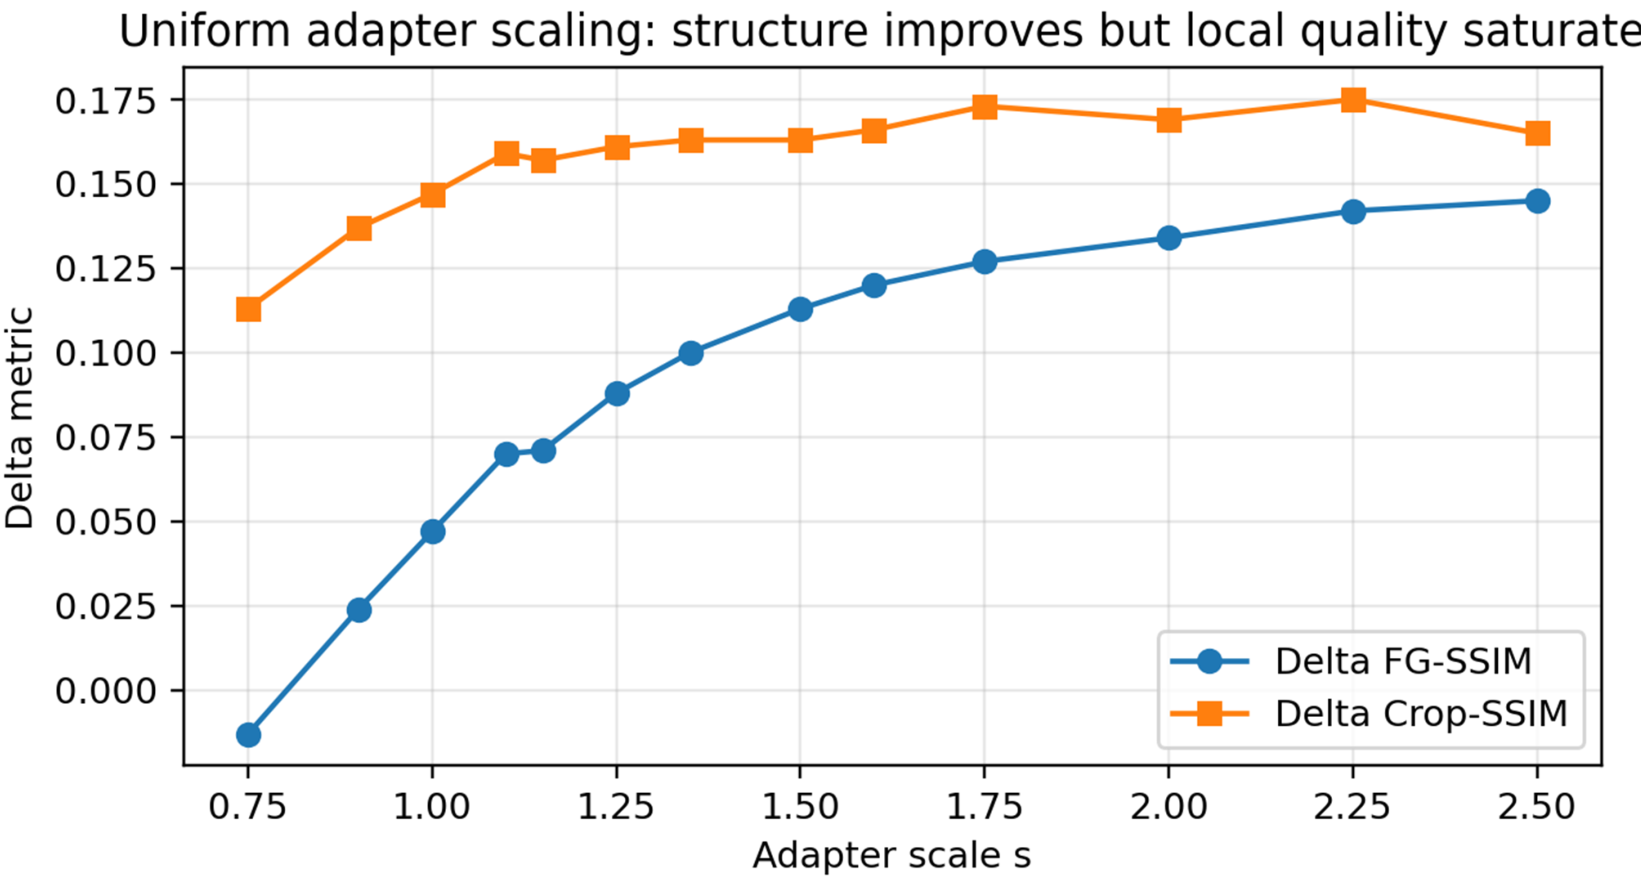
\includegraphics[width=\columnwidth]{fig2.pdf}
\caption{Historical fixed-scale diagnostic from the submitted 01549 paper. The plotted source reports FG-SSIM and Crop-SSIM over adapter scales; the underlying object-level run records are not available for independent reanalysis. It motivates measuring more than one endpoint, but is not a current confirmatory result.}
\label{fig:curve}
\end{figure}

The submitted heatmap depicts object-level variation across the reported scales, but its underlying rows cannot be reconstructed from the current evidence archive. We retain the visual diagnostic as part of the 01549 research history and do not infer a population-level response distribution from it. The updated Fresh C analysis below uses its own frozen cohort and matched inputs.

\begin{figure}[t]
\centering
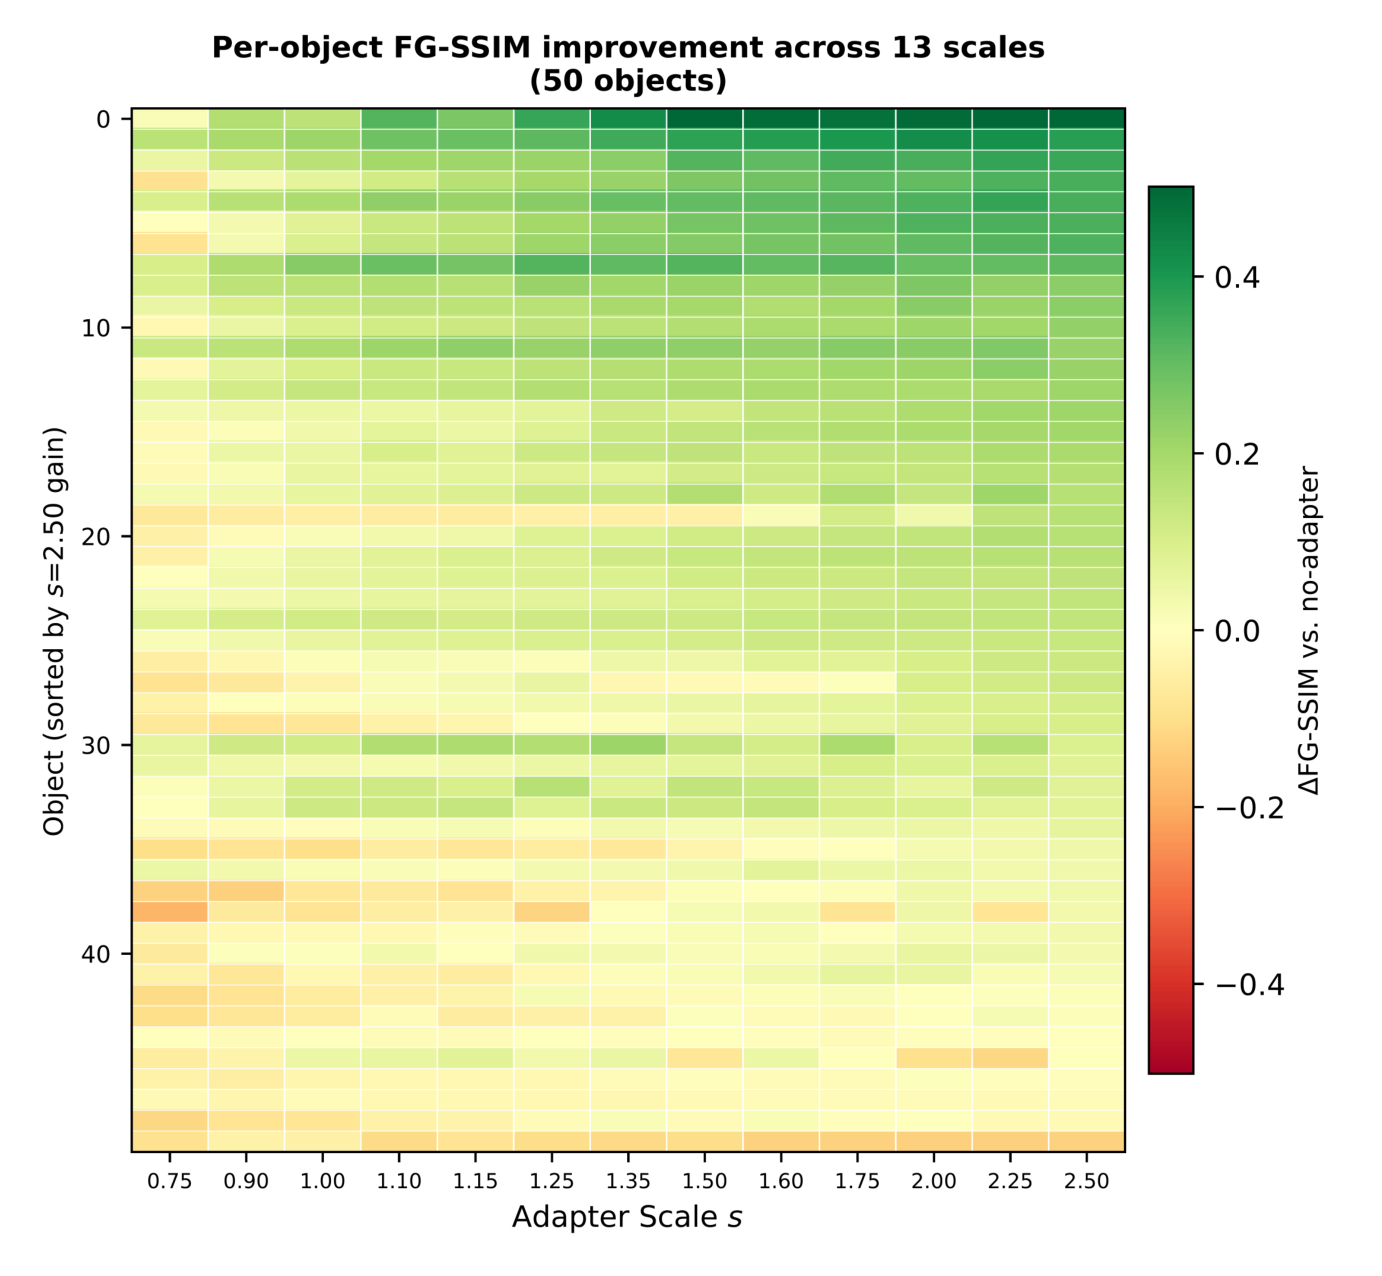
\includegraphics[width=\columnwidth]{fig3.pdf}
\caption{Historical per-object $\Delta$FG-SSIM heatmap reproduced from the 01549 submission (50 objects, 13 scales). The plot illustrates the originally reported response variation; row-level provenance is incomplete, so it is not used for a current population inference.}
\label{fig:heatmap}
\end{figure}

\subsection{Full-Object Appearance Evidence and Texture-Metric Scope}
\label{subsec:visual}

The submitted 26-object texture audit and its quantitative Figure~5 cannot be re-traced to object IDs, selection criteria, raw values, and an executable metric definition in the current evidence archive. We therefore remove its 92\% prevalence statement, its “true shape gain” classification, and its RGB-standard-deviation/gradient ratios from the scientific claims. Those statistics would describe variation, not texture fidelity, even if their source records were complete.

Figure~\ref{fig:qualitative} restores the original Fig.~4 role of showing full-object appearance beside a clearly marked local texture region. It compares the reference with GFL, GFH, and C3 for one selected C3--GFL favorable case and one adverse case; every column uses the same target view and pixel ROI within its object. Figure~\ref{fig:c3compare} retains the original C3-versus-fixed-scale question and adds a separate Generic Linear counterexample. These are selected Fresh C RGB illustrations, not a prevalence estimate or a texture-fidelity test. The full six-view, seven-condition panels, including No Adapter and LLH, remain in Supplementary Figure~S1.

\begin{figure*}[t]
\centering
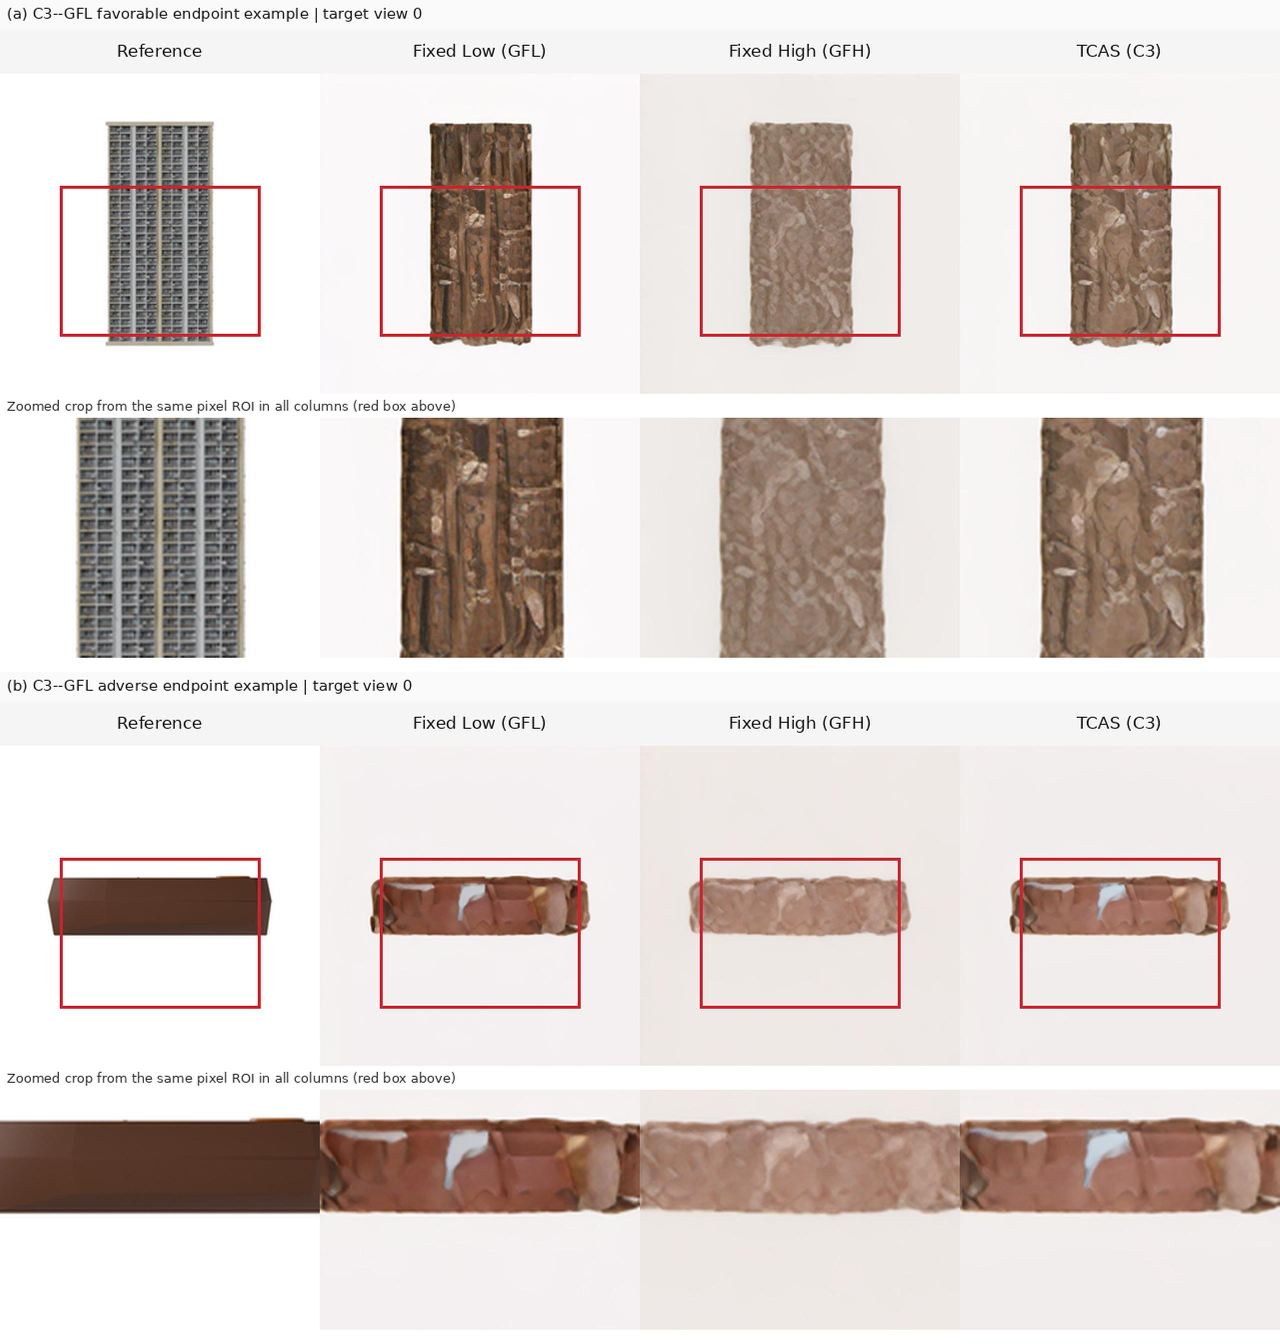
\includegraphics[width=\textwidth]{figures/fig4_freshc_context_roi.pdf}
\caption{Matched Fresh C comparisons under the same frozen object, reference, camera view, checkpoint, runner, seed policy, and inference protocol. Columns show the reference, fixed-low GFL, fixed-high GFH, and TCAS C3. Each panel shows the full target-view context with the shared ROI marked in red, followed by the same-pixel crop. Case (a) is selected because the paired C3--GFL FG-PSNR and FG-LPIPS differences both favor C3; case (b) is an adverse case in which both endpoints favor GFL. The outcome-selected examples are illustrative only and do not estimate case frequency or texture fidelity. The shown images are target-view RGB outputs, not baked textures, unseen-view renders, PBR results, or human-preference evidence. Model credits are in Supplementary Table~S1; source-image hashes and ROI coordinates are in the Fresh C figure manifest.}
\label{fig:qualitative}
\end{figure*}

\subsection{Timestep-Conditioned Adapter Scaling: Shape-Texture Balance of C3}
\label{subsec:c3}

The submitted paper records 17 uniform, layer-wise, and timestep-conditioned variants on a 24-object development probe and identifies C3 as its chosen profile. This study question remains relevant: does a stage-dependent request offer a useful control setting beyond a single global scale? Because the complete historical row-level data and selection provenance are not available in the current authority, the original Table~\ref{tab:probe} and Figure~\ref{fig:pareto} are retained as historical development records, not as a verified ranking or proof of optimality. Fresh C evaluates the recorded C3 profile without another schedule search.

\begin{table}[t]
\centering
\caption{Representative values reported for the historical 24-object, 17-variant development probe. The full candidate set is shown in Figure~\ref{fig:pareto}. The underlying row-level outputs and selection-time provenance are not available for independent reanalysis; the table records the submitted development result and does not establish an optimum.}
\label{tab:probe}
\footnotesize\setlength{\tabcolsep}{3pt}
\begin{tabular}{llcc}
\toprule
Variant & Reported category & $\Delta$FG-SSIM & $\Delta$Lap Var \\
\midrule
C4 & Late-stage high & 0.105 & $-$0.0120 \\
C2 & Timestep schedule & 0.104 & $-$0.0110 \\
B2 & Layer-wise schedule & 0.090 & $-$0.0135 \\
A\_s2.00 & Uniform & 0.087 & $-$0.0062 \\
C3 & Mid-stage high & 0.084 & $-$0.0006 \\
A\_s2.25 & Uniform & 0.079 & $-$0.0096 \\
A\_s2.50 & Uniform & 0.078 & $-$0.0108 \\
B6 & Layer-wise schedule & 0.000 & $-$0.0027 \\
\bottomrule
\end{tabular}
\end{table}

The original table and plot use shape and texture-variation proxies to describe the development choice. They do not establish that texture was faithful to the reference, nor that C3 was the unique best candidate. In this revision, C3 is therefore described as the historical profile carried forward for matched evaluation, not as a theorem-derived or globally optimal schedule.

The requested profile is piecewise constant over normalized sampling progress $p$:
\begin{equation}
s_{\mathrm{req}}(p) =
\begin{cases}
1.25, & 0 \le p < 1/3,\\
2.50, & 1/3 \le p < 2/3,\\
1.25, & 2/3 \le p \le 1,
\end{cases}
\qquad \mathrm{C3}=(1.25,2.50,1.25).
\end{equation}
This is an inference-time instruction on the existing adapter path; no weights are trained. Its tested value is task- and implementation-specific. The schedule operation itself is not claimed as a new general primitive.

Figure~\ref{fig:c3compare} presents compact Fresh C full-object and local-detail comparisons for the original C3-versus-fixed-scale question and the Generic Linear counter-result. The object-paired estimates in Section~\ref{subsec:largescale} carry the quantitative comparison.

\begin{figure*}[t]
\centering
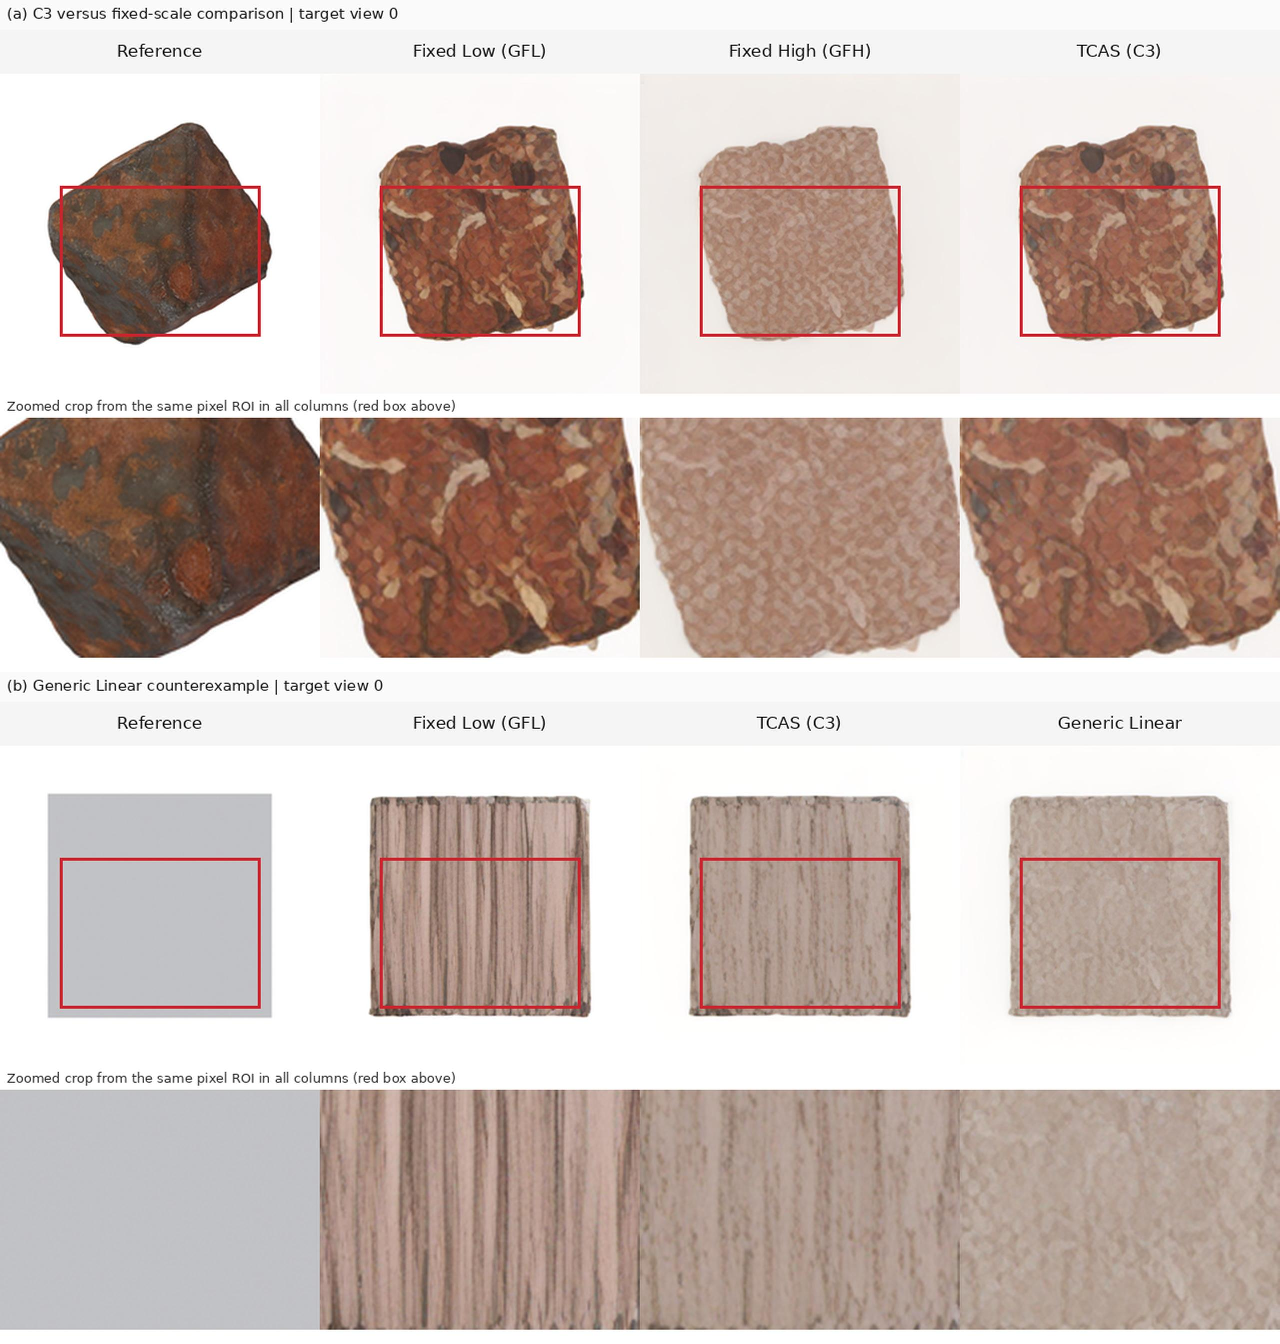
\includegraphics[width=\textwidth]{figures/fig5_freshc_context_roi.pdf}
\caption{Matched Fresh C comparisons under the same frozen object, reference, camera view, checkpoint, runner, seed policy, and inference protocol. (a) Reference, fixed-low GFL, fixed-high GFH, and C3 preserve the original fixed-scale comparison question; the selected object illustrates an endpoint trade-off between C3 and GFH. (b) Reference, GFL, C3, and Generic Linear show a counterexample in which both object-level FG-PSNR (C3 minus Generic Linear $=-3.491$~dB) and FG-LPIPS ($=+0.08172$) favor Generic Linear. Each context image marks the same pixel ROI used for the crop below. The examples were selected by outcome, so they do not estimate prevalence or establish a general winner or texture fidelity. Full six-view comparisons remain in Supplementary Figure~S1. Attribution is in Supplementary Table~S1; input and ROI hashes are in the Fresh C figure manifest.}
\label{fig:c3compare}
\end{figure*}

\begin{figure}[!t]
\centering
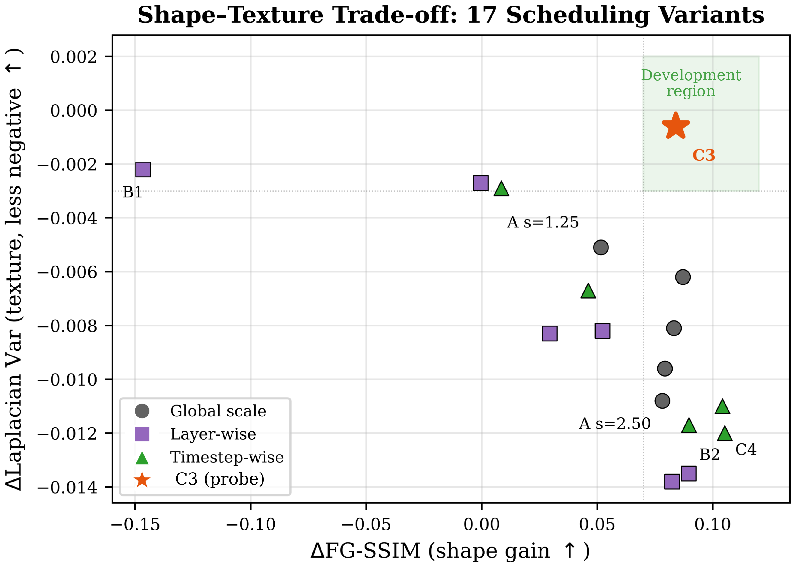
\includegraphics[width=\columnwidth]{figures/fig7_c3_development.pdf}
\caption{Historical 17-variant shape--texture development plot from the submitted 01549 paper, restricted to the 24-object development probe and not an independent validation set. The plot labels have been locally changed to “Development region” and “C3 (probe)” to identify their development-set role; neither the shaded region nor C3 denotes a unique optimum, a texture-fidelity ranking, or a general schedule law. The underlying row-level candidate outputs are not available for independent reanalysis.}
\label{fig:pareto}
\end{figure}

The source Figure~5 (26-object texture ratios) is not included as an active result because its object IDs, selection trace, and metric lineage are incomplete. The original 24-object Table~3 is moved to Supplementary Section S10 as a verbatim historical diagnostic, with no texture-fidelity or population inference. Both source assets remain preserved in the authenticated submission and forensic archive; neither decision removes the fixed-scale research question or the development record of C3.

\subsection{Large-Scale Matched Image-Space Evaluation}
\label{subsec:largescale}

Fresh C is a revision-era matched image-space study on $N=300$ objects. Its primary run contains No Adapter, global fixed-low (GFL), global fixed-high (GFH), and the historical C3 profile. A separate addendum evaluates Generic Linear and a layer-conditioned low--high--low profile (LLH) on the same 300 object identifiers; it is not an independent cohort. All conditions within a run share the object, reference/target inputs, six target views, initial latents, and seed. Object is the inferential unit, with views averaged within object.

The registered primary contrast is C3 minus GFL on foreground PSNR (FG-PSNR). The point estimate is $+0.522352$~dB (95\% percentile-bootstrap CI $[+0.404160,+0.640669]$); C3 is higher on 206/300 objects (68.7\%), with median paired difference $+0.554514$~dB. Registered secondary endpoints are reported with the multiplicity treatment and full paired statistics in Supplementary Section S2. PSNR, LPIPS, and SSIM quantify image-space agreement on their respective endpoints; they are not direct measures of texture fidelity or 3D material quality.

This primary contrast changes more than temporal placement. Across the 50 steps, the applied deep and middle scale sums are 82.5 each for C3 and 62.5 each for GFL; the shallow sum is 40 for both after the native 0.8 cap. The Fresh C estimate therefore supports the recorded C3 intervention relative to GFL under this wrapper, but cannot be attributed to timing alone or interpreted as a pure schedule-shape effect.

\begin{table*}[t]
\centering
\caption{Fresh C image-space condition means. The primary run contains No Adapter, GFL, GFH, and C3. Generic Linear and LLH are revision-era addendum conditions evaluated on the same object identifiers, not a second independent cohort. Values are means of object-level metrics over six target views.}
\label{tab:freshc-absolute}
\scriptsize\setlength{\tabcolsep}{4pt}
\begin{tabular}{lccccc}
\toprule
Method & $N$ & FG-PSNR$\uparrow$ & FG-LPIPS$\downarrow$ & FG-SSIM$\uparrow$ & Edge-SSIM$\uparrow$ \\
\midrule
\multicolumn{6}{l}{Primary run} \\
No Adapter & 300 & 6.9779 & 0.2288 & 0.4086 & 0.4314 \\
GFL & 300 & 11.3077 & 0.2051 & 0.3500 & 0.4728 \\
GFH & 300 & 12.5777 & 0.1891 & 0.4201 & 0.4961 \\
C3 (TCAS) & 300 & 11.8301 & 0.1998 & 0.3746 & 0.4773 \\
\midrule
\multicolumn{6}{l}{Same-cohort revision-era addendum} \\
Generic Linear & 300 & 12.4230 & 0.1862 & 0.4026 & 0.4880 \\
LLH & 300 & 12.4506 & 0.1876 & 0.3911 & 0.4863 \\
\bottomrule
\end{tabular}
\end{table*}

\begin{table*}[t]
\centering
\caption{Fresh C paired differences, condition A minus B. Cells report the mean difference and pointwise 95\% object-bootstrap CI. Positive PSNR/SSIM and negative LPIPS differences favour A. C3--No Adapter and C3--GFH are post-hoc contrasts; the addendum shares the primary run's object identifiers. Multiplicity-adjusted tests and the full endpoint family are in Supplementary Section S2.}
\label{tab:freshc-contrasts}
\scriptsize\setlength{\tabcolsep}{3pt}
\begin{tabular}{lcccc}
\toprule
Contrast & FG-PSNR (dB) & FG-LPIPS & FG-SSIM & Edge-SSIM \\
\midrule
C3 $-$ GFL & $+0.522\ [0.404,0.641]$ & $-0.005345\ [-0.006326,-0.004403]$ & $+0.02453\ [0.02120,0.02805]$ & $+0.004494\ [0.003411,0.005586]$ \\
C3 $-$ No Adapter & $+4.852\ [4.553,5.142]$ & $-0.02905\ [-0.03352,-0.02464]$ & $-0.03401\ [-0.04214,-0.02591]$ & $+0.04586\ [0.04114,0.05054]$ \\
C3 $-$ GFH & $-0.748\ [-0.885,-0.609]$ & $+0.01070\ [0.008958,0.012513]$ & $-0.04553\ [-0.04937,-0.04167]$ & $-0.01881\ [-0.02084,-0.01683]$ \\
C3 $-$ Generic Linear & $-0.593\ [-0.837,-0.351]$ & $+0.01351\ [0.01160,0.01549]$ & $-0.02810\ [-0.03197,-0.02439]$ & $-0.01069\ [-0.01300,-0.00850]$ \\
LLH $-$ C3 & $+0.621\ [0.391,0.855]$ & $-0.01214\ [-0.01386,-0.01048]$ & $+0.01658\ [0.01311,0.02003]$ & $+0.009033\ [0.006867,0.011296]$ \\
LLH $-$ Generic Linear & $+0.028\ [-0.015,0.070]$ & $+0.001372\ [0.000762,0.002081]$ & $-0.01152\ [-0.01337,-0.00996]$ & $-0.001660\ [-0.002096,-0.001256]$ \\
\bottomrule
\end{tabular}
\end{table*}

The C3--GFL comparison supports a bounded statement: on this frozen, UID-disjoint cohort and image-space endpoint, the recorded C3 intervention improves mean FG-PSNR relative to GFL. The paired conditions use one frozen checkpoint, common runner, seed policy, inputs, target views, metrics, and recorded native-cap semantics. The historical 01549 v1/v2 checkpoint distinction is preserved, and Fresh C is not presented as a numerical reproduction of the old Table~4 result. This historical difference does not alter the internal pairing or held-out status of Fresh C.

The counter-results delimit that finding. GFH has more favorable cohort means than C3 on all four displayed endpoints. Generic Linear also has more favorable means than C3 on all four; for C3 minus Generic Linear, the mean FG-PSNR difference is $-0.593$~dB (95\% CI $[-0.837,-0.351]$), although the median is $+0.073956$~dB and C3 is higher on 155/300 objects (51.7\%). LLH's FG-PSNR mean exceeds C3 by $+0.621$~dB, while its median difference is $-0.153$~dB and only 140/300 objects favour LLH; its lower mean FG-LPIPS favours LLH. For LLH versus Generic Linear, the FG-PSNR CI includes zero, which is not evidence of equivalence; the FG-LPIPS difference favours Generic Linear. The endpoint means and object-level distributions do not identify a universal winner.

Fresh C contains no validated texture-variation or texture-fidelity endpoint. We therefore do not revive the original 300-object RGB/Laplacian/gradient tables or their “retention” interpretation. In those diagnostics, a larger response could represent meaningful detail or an artifact; it cannot by itself establish fidelity.

\subsection{First-round cluster-aware preference study}
\label{subsec:preference}

The 01549 first-round revision reported a blinded three-alternative forced-choice study on 30 objects with 24 participants. Participants compared conservative fixed-scale, aggressive fixed-scale, and C3 outputs for texture naturalness, shape consistency, and overall quality; condition order was randomized per trial. Each criterion had 720 first-choice decisions. Table~\ref{tab:preference} reports the aggregate counts; participant-level responses are not redistributed with this revision.

\begin{table}[t]
\centering\footnotesize
\caption{First-round 01549 3AFC results retained as reported. Percentages use 720 decisions per criterion; preference is not a measure of reference texture fidelity.}
\label{tab:preference}
\begin{tabular}{lccc}
\toprule
Method & Texture naturalness & Shape consistency & Overall quality \\
\midrule
$s=1.25$ & 332/720 (46.1\%) & 96/720 (13.3\%) & 176/720 (24.4\%) \\
$s=2.50$ & 104/720 (14.4\%) & 331/720 (46.0\%) & 126/720 (17.5\%) \\
C3 (TCAS) & 284/720 (39.4\%) & 293/720 (40.7\%) & 418/720 (58.1\%) \\
\bottomrule
\end{tabular}
\end{table}

The reported analysis used a two-level participant/object bootstrap with 10,000 resamples. C3's overall-quality share was 58.1\% (95\% CI [50.1\%, 65.8\%]); its differences from the conservative and aggressive baselines were +33.6 points (CI [19.3, 47.2]) and +40.6 points (CI [29.4, 51.8]). The single-criterion advantages for texture naturalness and shape consistency had intervals crossing zero. This bounded preference result does not validate texture fidelity, unseen-view quality, or the Fresh C cohort.

\subsection{FAC controlled re-examination reported in 01549}
\label{subsec:facreported}

A controlled re-examination of Full Adaptive Correction (FAC) was previously reported, with the base model, VAE, and GeoTex-Adapter frozen and roughly $6\times10^3$ controller parameters trainable. The stated protocol used the enhanced latent denoising objective (foreground weight 1.7, edge weight 1.3, and a latent-SSIM term), AdamW at peak learning rate $10^{-4}$ with 100 warm-up steps, and 2,000 training steps on a training pool reported as 1,706 objects and disjoint from evaluation. It reported a 300-object paired evaluation: every trained configuration reduced FG-PSNR versus TCAS by 1.10--2.94 dB, with at most 48/300 wins; the untrained C3-envelope control on 12 objects had $\Delta$FG-PSNR $=-0.18$ dB (95\% CI [$-0.42,+0.05$]). The seven reported configurations and endpoint values are retained in Supplementary Table~S11.

These FAC outcomes are retained as previously reported results. They are not presented as a new 1008 training run. The current archive audit found that a recovered configuration points to a 1,200-object list rather than the 1,706-object pool stated in 01549, and does not bind the training seed and run outputs in one manifest. We therefore disclose the remaining reproducibility gap and make no code-release claim; TCAS remains the sole training-free method.

\subsection{Stage Sensitivity and Applicability Boundaries}
\label{subsec:stageboundaries}

A separate post-inspection strict-276 follow-up compares temporal profiles on the clean-v2 276-object cohort under the checkpoint SHA recorded for Fresh C. C3 and temporal L--L--H have near-matched, but not identical, applied-scale sums: 82.5 versus 83.75 for each of the deep and middle groups, with 40 for each shallow group. Post-scale residual-norm dose is not matched. In this run, the C3-minus-temporal-L--L--H FG-PSNR difference is $-0.177084$~dB (95\% CI $[-0.230539,-0.130784]$), and, in this post-inspection stage-placement experiment, temporal L--L--H outperforms C3 on all six formal endpoints. Against the fixed-mean profile, C3's FG-PSNR difference is $+0.502875$~dB (95\% CI $[+0.462018,+0.542244]$). The post-inspection follow-up is not an independent cohort replication and does not identify an equal-realized-dose causal effect or establish an optimal schedule. Full comparisons are in Supplementary Table S7.

The A2/A3b layer-window maps detect response heterogeneity under their tested bounded interventions. A3b has zero common-support rows across its three layer groups among 2,250 layer-step observations, so dose adjustment cannot identify a dose-independent layer-by-time mechanism. Fresh B is a separate 150-object cohort; its temporal LLH result is not a replication of C3. Core-7 is a retrospective seven-condition summary on the same clean-v2 276-object list and checkpoint SHA as Fresh C, assembled from condition records that do not establish one common runner or complete input-tensor identity. Its stored object-level metrics show C3--GFH $+0.725229$~dB Full-PSNR but $-1.214235$~dB FG-PSNR (nominal pointwise 95\% CIs $[+0.647134,+0.806467]$ and $[-1.313952,-1.114705]$, respectively). These endpoint-opposed estimates are retained as a retrospective diagnostic in Supplementary Section S5, not as confirmatory R1.2 evidence or a reproduction of the original $+0.96$~dB estimate. The separate \texttt{MAIN-STAGE-276} profile-placement run uses the same clean-v2 object cohort/checkpoint lineage and is not independent of these diagnostics. The 01549 first-round adapter-dependence analysis is also retained in the Supplement. The MV-Adapter probe analyzed 98 of 99 planned objects; the omitted frozen GLB contains path geometry but no triangle faces. Its production additive-residual bootstrap has an invalid zero-power null and is not used for interaction inference. A post hoc exploratory object-cluster robust Wald audit (8 degrees of freedom) found no interaction surviving Holm correction across four metrics: FG-LPIPS $p=0.101$, PSNR $p=0.434$, FG-SSIM $p=0.039$ nominal and $p=0.156$ after correction, and CIEDE2000 $p=0.862$. The tested 0.75--1.00 intervention range showed only small late-window shallow FG-LPIPS worsening and did not reproduce the broad GeoTex response. This bounded analysis does not establish absence of interaction or equivalence. The MVDiffusion probe covered 75 objects through a different correspondence-aware interface and produced mixed or negative endpoint results. These are actual cross-backbone interface probes, but they do not share a matched conditioning path or runner and therefore do not establish general transfer (Supplementary Section S5).

The historical N=20 GLB-native unseen-view check used unlit base color on a UV-compatible subset and produced mixed endpoint results. It is a bounded 3D rendering observation only; it does not establish full PBR, seam, or population-level texture superiority (Supplementary Table S8). Fresh C's attempted 24-object bake did not pass the native-input gate, so no new bake or seam outcome is reported.

\section{Limitations}
\label{sec:limitations}

Fresh C is a held-out 300-object comparison whose conditions share one frozen checkpoint, runner, seed policy, inputs, metric implementation, and recorded native-cap semantics. The checkpoint is a controlled retraining and differs from the v1 path named for 01549 Table~4; the 01549 Table~9/FAC work uses a separate v2 strong-residual adapter. These historical v1/v2 differences are reported separately from the within-Fresh-C paired comparison. Fresh C does not numerically reproduce the old $+0.96$~dB Table~4 estimate. The historical main-table endpoint implementation is not recoverable for a numerical equivalence claim. Core-7 and the post-inspection strict-276 profile-placement analysis use the clean-v2 276-object list and the checkpoint SHA recorded for Fresh C, but are separate runs from Fresh C; Core-7 condition records do not establish one shared runner or complete input-tensor identity. They remain retrospective supporting diagnostics rather than confirmatory comparisons.

Texture variation and texture fidelity are distinct. The submitted RGB standard deviation, Laplacian variance, and gradient summaries are not re-used as fidelity measures; their source records and definitions are incomplete, and such metrics can rise with artifacts. Fresh C reports PSNR, LPIPS, and SSIM endpoints but has no validated texture-fidelity measure. The 01549 cluster-aware preference study is a separate subjective choice result, not a fidelity or 3D-quality endpoint. Fresh C has no validated baked-mesh, seam, or PBR measure. Historical N=20 unlit base-color renders provide only a small, mixed unseen-view result.

An exploratory four-object color-pathway audit found that changing the global appearance embedding can shift chroma. A separate Fresh B input-only audit found that stored embeddings matched neither of the two compared source-conditioning reconstructions within 0.03 for 150/150 inputs. This makes cache/source alignment a plausible contributor, not an established general cause of color drift. The C1 chroma-anchor candidate met its numeric gate (mean unseen-view $\Delta$FG-CIEDE2000 $=-1.5602$, 95\% CI [$-2.2621,-0.6299$], four of four) but failed the locked visual gate: one case showed no clear gain, and another retained mismatch with a faint cyan/blue rim. B2's selected raw-source embedding substitution did not meet its numeric gate (mean object-level change in the lower-is-better $\Delta$FG-CIEDE2000 endpoint $=+0.1729$, 95\% CI [$-0.2044,+0.6810$], one of four improved) and showed no clear visual correction. No independent Fresh B repair validation was performed. These development findings identify a control pathway and a plausible contributor, not a validated correction or a complete root cause.

The requested TCAS profile does not uniquely determine the applied scale or correction magnitude. Fresh C's native wrapper caps shallow requests at 0.8, and residual norms depend on the adapter output. The strict-276 schedule sums are only approximately matched and do not equalize realized dose; A3b has no cross-layer common support. These data do not identify a dose-independent mechanism, an optimal selector, or a schedule that dominates all endpoints and objects.

We withdraw the CAI optimality proposition and the earlier positive FAC extension claim; the negative FAC controlled re-examination and the cluster-aware 01549 preference study are retained as previously reported first-round results with their stated scope and provenance limits. The old pooled $+0.96$~dB headline and broad texture-retention claim are not used as current evidence. CLIP-IQA is not used to establish texture fidelity. The revised claim boundaries are documented in the changelog.

\section{Conclusion}
\label{sec:conclusion}

Adapter strength is an inference-time control over the geometry residual used during multi-view image generation. TCAS makes that control explicit as a requested temporal profile on the existing GeoTex-Adapter path; C3, $(1.25,2.50,1.25)$, is the profile evaluated here, not a general scheduling rule.

On the matched 300-object Fresh C cohort, C3 exceeds GFL by $+0.522352$~dB on the registered FG-PSNR endpoint (95\% CI $[+0.404160,+0.640669]$). GFH and Generic Linear have more favorable means than C3 on all four displayed endpoints. C3 also applies larger deep/middle scale sums than GFL (82.5 versus 62.5 per layer; both apply 40 in shallow), so the primary contrast does not isolate temporal scheduling from applied scale.

The separate strict-276 placement follow-up shows that the measured response changes across tested profiles: C3 exceeds the fixed-mean profile by $+0.502875$~dB FG-PSNR, while temporal L--L--H exceeds C3 by $0.177084$~dB FG-PSNR and is favored on all six formal endpoints. Layer-window analyses also detect response heterogeneity, but their dose and common-support limits do not identify an equal-dose mechanism. The cross-interface probes do not establish general transfer.

The contribution is a task-specific specification and matched evaluation of a training-free control on the GeoTex residual path. It makes the requested profile, wrapper-applied scale under native caps, and resulting residual magnitude explicit, then compares the recorded intervention with fixed and scheduled controls on paired image-space endpoints. The evidence does not establish texture fidelity, baked-texture quality, seam consistency, PBR appearance, cross-backbone transfer, or a universally preferred schedule.

\section*{Data availability}

All data included in this study are available upon request by contact with the corresponding author.

\section*{Declaration of competing interests}

The authors declare that they have no known competing financial interests or personal relationships that could have appeared to influence the work reported in this paper.


\begin{thebibliography}{45}
\bibitem{liu2023zero1to3}
Liu R, Wu R, Van Hoorick B, et al. Zero-1-to-3: Zero-shot one image to 3D object. \textit{Proceedings of the IEEE/CVF International Conference on Computer Vision}, 2023.

\bibitem{shi2023zero123pp}
Shi R, Chen H, Zhang Z, et al. Zero123++: A single image to consistent multi-view diffusion base model. arXiv:2310.15110, 2023.

\bibitem{liu2023syncdreamer}
Liu Y, Lin C, Zeng Z, et al. SyncDreamer: Generating multiview-consistent images from a single-view image. \textit{International Conference on Learning Representations}, 2024.

\bibitem{long2023wonder3d}
Long X, Guo Y C, Lin C, et al. Wonder3D: Single image to 3D using cross-domain diffusion. \textit{Proceedings of the IEEE/CVF Conference on Computer Vision and Pattern Recognition}, 2024.

\bibitem{shi2024mvdream}
Shi Y, Wang P, Ye J, et al. MVDream: Multi-view diffusion for 3D generation. \textit{International Conference on Learning Representations}, 2024.

\bibitem{wang2023imagedream}
Wang P, et al. ImageDream: Image-prompt multi-view diffusion for 3D generation. arXiv:2312.02201, 2023.

\bibitem{xu2024instantmesh}
Xu J, et al. InstantMesh: Efficient 3D mesh generation from a single image with sparse-view large reconstruction models. \textit{Advances in Neural Information Processing Systems}, 2024.

\bibitem{ke2024era3d}
Li P, Liu Y, Long X, et al. Era3D: High-resolution multiview diffusion using efficient row-wise attention. \textit{Advances in Neural Information Processing Systems}, 2024.

\bibitem{chen2023text2tex}
Chen D Z, et al. Text2Tex: Text-driven texture synthesis via diffusion models. \textit{Proceedings of the IEEE/CVF International Conference on Computer Vision}, 2023.

\bibitem{richardson2023texture}
Richardson E, Metzer G, Alaluf Y, et al. TEXTure: Text-guided texturing of 3D shapes. \textit{ACM SIGGRAPH 2023 Conference Proceedings}, 2023.

\bibitem{poole2023dreamfusion}
Poole B, Jain A, Barron J T, Mildenhall B. DreamFusion: Text-to-3D using 2D diffusion. \textit{International Conference on Learning Representations}, 2023.

\bibitem{chen2023fantasia3d}
Chen R, Chen Y, Jiao N, Jia K. Fantasia3D: Disentangling geometry and appearance for high-quality text-to-3D content creation. \textit{Proceedings of the IEEE/CVF International Conference on Computer Vision}, 2023.

\bibitem{shao2025mvpainter}
Shao M, Xiong F, Sun Z, Xu M. MVPainter: Accurate and detailed 3D texture generation via multi-view diffusion with geometric control. arXiv:2505.12635, 2025.

\bibitem{kynkanniemi2024limited}
Kynk\"a\"anniemi T, Aittala M, Karras T, et al. Applying guidance in a limited interval improves sample and distribution quality in diffusion models. \textit{Advances in Neural Information Processing Systems}, 2024.

\bibitem{perla2026survey}
Perla S R K, Zhang H, Mahdavi-Amiri A. Advances in neural 3D mesh texturing: A survey. \textit{Computer Graphics Forum}, 2026, e70392.

\bibitem{guzman2026adaptive}
Guzm\'an J E, Mould D, Paquette E. Adaptive multiresolution exemplar-based texture synthesis on animated fluids. \textit{Computers \& Graphics}, 2026, 134: 104490.

\bibitem{lv2025interpretable}
Lv X, Wu Z, Xu J, et al. Interpretable procedural material graph generation via diffusion models from reference images. \textit{The Visual Computer}, 2025, 41(13): 11195--11205.

\bibitem{zeng2024paint3d}
Zeng X, Chen X, Qi Z, et al. Paint3D: Paint anything 3D with lighting-immersive texture generation. \textit{Proceedings of the IEEE/CVF Conference on Computer Vision and Pattern Recognition}, 2024.

\bibitem{cheng2024mvpaint}
Cheng W, Mu J, Zeng X, et al. MVPaint: Synchronized multi-view diffusion for painting anything 3D. \textit{Proceedings of the IEEE/CVF Conference on Computer Vision and Pattern Recognition}, 2025.

\bibitem{lai2025hunyuan3d}
Zhao Z, Lai Z, Lin Q, et al. Hunyuan3D 2.0: Scaling diffusion models for high resolution textured 3D assets generation. arXiv:2501.12202, 2025.

\bibitem{huang2024mvadapter}
Huang Z, et al. MV-Adapter: Multi-view consistent image generation made easy. \textit{Proceedings of the IEEE/CVF International Conference on Computer Vision}, 2025.

\bibitem{liu2024synchronized}
Liu Y X, Xie M S, Liu H Y, Wong T T. Text-guided texturing by synchronized multi-view diffusion. \textit{SIGGRAPH Asia 2024 Conference Papers}, 2024.

\bibitem{xu2026wondertex}
Xu Q, Han X G, Zhang L. WonderTex: Consistent-and-seamless texture generation with text-guided multi-view image diffusion models. \textit{IEEE Transactions on Visualization and Computer Graphics}, 2026, 32(7): 5815--5825.

\bibitem{mou2023t2iadapter}
Mou C, Wang X, Xie L, et al. T2I-Adapter: Learning adapters to dig out more controllable ability for text-to-image diffusion models. \textit{Proceedings of the AAAI Conference on Artificial Intelligence}, 2024.

\bibitem{zhang2023controlnet}
Zhang L, Rao A, Agrawala M. Adding conditional control to text-to-image diffusion models. \textit{Proceedings of the IEEE/CVF International Conference on Computer Vision}, 2023.

\bibitem{ye2023ipadapter}
Ye H, Zhang J, Liu S, Han X, Yang W. IP-Adapter: Text compatible image prompt adapter for text-to-image diffusion models. arXiv:2308.06721, 2023.

\bibitem{hu2022lora}
Hu E J, Shen Y, Wallis P, et al. LoRA: Low-rank adaptation of large language models. \textit{International Conference on Learning Representations}, 2022.

\bibitem{liu2024dora}
Liu S Y, Wang C Y, Yin H, et al. DoRA: Weight-decomposed low-rank adaptation. \textit{International Conference on Machine Learning}, 2024.

\bibitem{zhang2023adalora}
Zhang Q, Zuo S, Liang C, et al. AdaLoRA: Adaptive budget allocation for parameter-efficient fine-tuning. \textit{International Conference on Learning Representations}, 2023.

\bibitem{kulkarni2026ssi}
Kulkarni A S, et al. Scheduled Style Injection: Expanding the Style-Content Pareto Frontier in Training-Free Diffusion-Based Style Transfer. \textit{Proceedings of the IEEE/CVF Conference on Computer Vision and Pattern Recognition Workshops (CVPRW), NTIRE Workshop}, 2026.

\bibitem{ho2020ddpm}
Ho J, Jain A, Abbeel P. Denoising diffusion probabilistic models. \textit{Advances in Neural Information Processing Systems}, 2020.

\bibitem{song2021ddim}
Song J, Meng C, Ermon S. Denoising diffusion implicit models. \textit{International Conference on Learning Representations}, 2021.

\bibitem{ho2022cfg}
Ho J, Salimans T. Classifier-free diffusion guidance. \textit{NeurIPS Workshop on Deep Generative Models and Downstream Applications}, 2021. arXiv:2207.12598.

\bibitem{castillo2023adaptive}
Castillo A, Kohler J, P\'erez J C, et al. Adaptive guidance: Training-free acceleration of conditional diffusion models. \textit{Proceedings of the AAAI Conference on Artificial Intelligence}, 2025.

\bibitem{wang2004ssim}
Wang Z, Bovik A C, Sheikh H R, Simoncelli E P. Image quality assessment: From error visibility to structural similarity. \textit{IEEE Transactions on Image Processing}, 2004, 13(4): 600--612.

\bibitem{zhang2018lpips}
Zhang R, Isola P, Efros A A, Shechtman E, Wang O. The unreasonable effectiveness of deep features as a perceptual metric. \textit{Proceedings of the IEEE/CVF Conference on Computer Vision and Pattern Recognition}, 2018.

\end{thebibliography}
\end{document}
